%%% Local Variables:
%%% mode: latex
%%% TeX-master: "main.tex"
%%% End:

\tikzstyle{bag} = [text width=10em, text centered]
\tikzstyle{end} = []
\begin{figure}[H]
  \centering
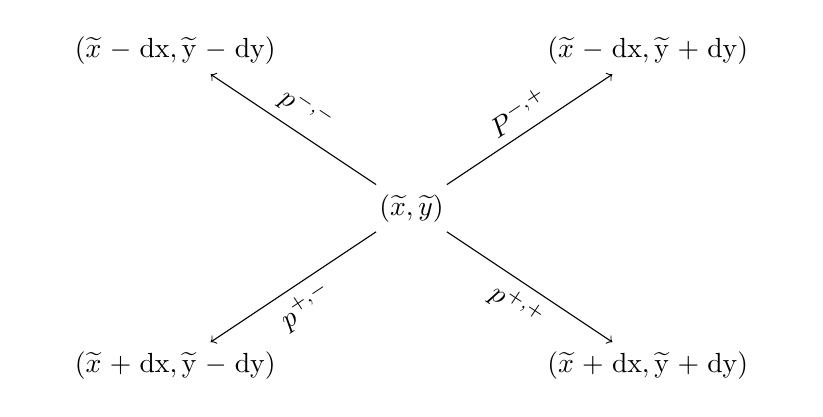
\begin{tikzpicture}[sloped]
  \node (xy) at (0,0) [bag] {$(\widetilde{x}, \widetilde{y})$};
  \node (a) at ( 3,-2) [bag] {$(\widetilde{x} + \rm{d}x, \widetilde{y} + \rm{d}y)$};
  \node (b) at ( -3,-2) [bag] {$(\widetilde{x} + \rm{d}x, \widetilde{y} - \rm{d}y)$};
  \node (c) at ( 3,2) [bag]{$(\widetilde{x} - \rm{d}x, \widetilde{y} + \rm{d}y)$};
  \node (d) at ( -3,2) [bag]{$(\widetilde{x} - \rm{d}x, \widetilde{y} - \rm{d}y)$};
  \draw [->] (xy) to node [below] {$p^{+, +}$} (a);
  \draw [->] (xy) to node [below] {$p^{+, -}$} (b);
  \draw [->] (xy) to node [above] {$P^{-, +}$} (c);
  \draw [->] (xy) to node [above] {$p^{-, -}$} (d);
\end{tikzpicture}
\end{figure}



